\chapter{Introduction into Part III}

We frequently worked in \parref{par:one} and \parref{par:two} with tensors, which have non-negative coordinates and occasionally are boolean (see \defref{def:booleanTensor}) or directed (see \defref{def:directedTensor}).
While boolean tensors have appeared as semantical representation of formulas, directed tensors have appeared mostly as conditional distributions.
In this chapter we provide further insights into the situation, where tensors satisfy both.
For a schematic depiction of this see \figref{fig:dbTensorSketch}.

\begin{figure}[h]
    \begin{center}
        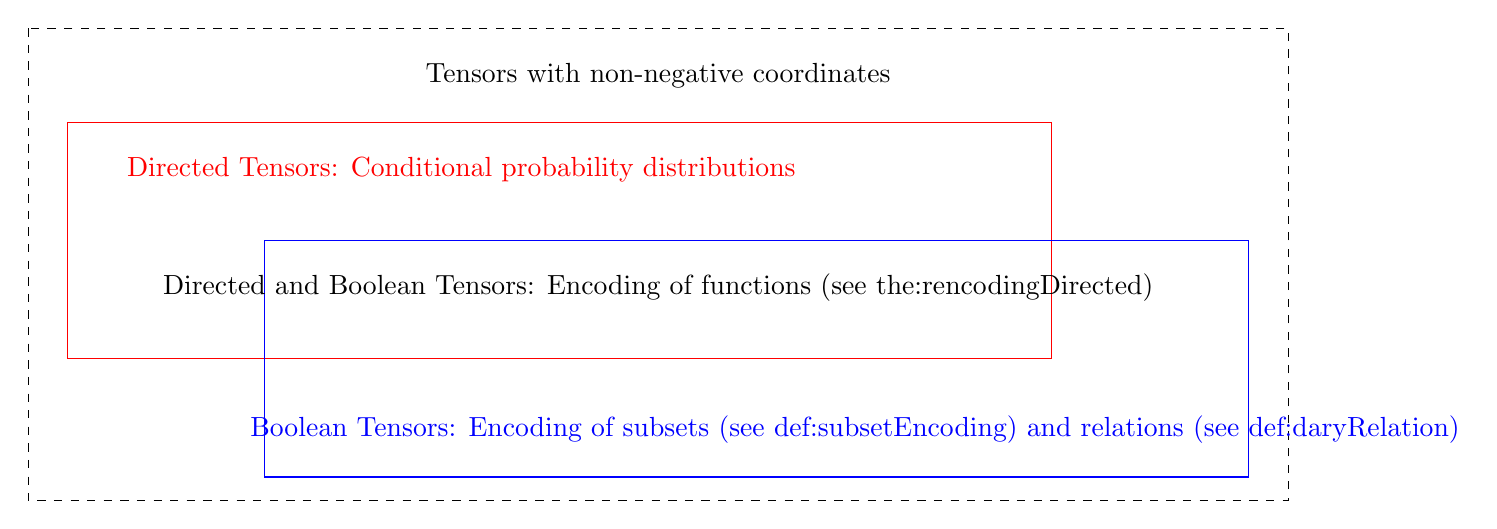
\begin{tikzpicture}[yscale=0.6]
	\draw[dashed] (-10.5,12) rectangle (5.5,2);
	\node[anchor=center] (text) at (-2.5,11) {Tensors with non-negative coordinates};
	
	\draw[red] (-10,10) rectangle (2.5,5); 
	\node[anchor=center,red] (text) at (-5,9) {Directed Tensors: Conditional probability distributions};
	\draw[blue] (-7.5,7.5) rectangle (5,2.5); 
	\node[anchor=center,blue] (text) at (0,3.5) {Boolean Tensors: Encoding of subsets (see \defref{def:subsetEncoding}) and relations (see \defref{def:daryRelation})};

	\node[anchor=center] (text) at (-2.5,6.5) {Directed and Boolean Tensors: Encoding of functions (see \theref{the:rencodingDirected})};
\end{tikzpicture}
    \end{center}
    \caption{Sketch of the tensors with non-negative coordinates.
    We investigate in this chapter tensors, which are directed and boolean.}\label{fig:dbTensorSketch}
\end{figure}